% UPDATED BY MARCUS SCHAGERBERG, 2023
% CREATED BY WOLFGANG AHRENDT, 2021


\section{Unity}
Unity is a cross-platform game engine used to create both 2D and 3D games. Unity supports a lot of features that speed up development time. 

\newcommand{\timeconstraint}{, \quad 0 \le t \le 1}
\newcommand{\lerp}{\rightarrow}
\newcommand{\p}[1]{P\textsubscript{#1}}

% Marcus Schagerberg
\section{Bézier curves}
    A Bézier curve is a parametric curve between two points, that curves according to a set of intermediate points. The points are called control points, where the first and last point are the endpoints of the curve. A linear Bézier curve only has two points, which means that it is a line between the points. It is defined by the following function:

    $$
        P(t) = (1-t)^2P_0 + 2t(1-t)P_1 + t^2P_2 \timeconstraint
    $$

    The parameter $t$ is the ratio along the line, with $t = 0$ and $t = 1$ marking the endpoints. This is what is known as linear interpolation in mathematics. A linear Bézier curve is therefore simply a linear interpolation between the points $P_0$ and $P_1$. Let's define this as $P_0 \lerp P_1$. The quadratic Bézier curve consists of two linear interpolations:
    
    $$ A) \quad P_0 \lerp P_1$$
    $$ B) \quad P_1 \lerp P_2 $$
    
    It is then defined as the linear interpolation between these points, i.e $ A \lerp B $. All linear interpolations in this case depend on the same $t$, which is what creates the curvature of the Bézier curves.

    Since a quadratic Bézier curve has three points, it will have two endpoints as well as an additonal control point between them. By moving the control point, the shape of the Bézier curve can be altered. This is presented with the following examples, the first three of which have static endpoints demonstrating how the middle control point can be used to form the curve. The final example eludes to the fact that the control points can be placed anywhere without the requirement of any order.

    \begin{figure}[H]
        \begin{tabular}{cc}
            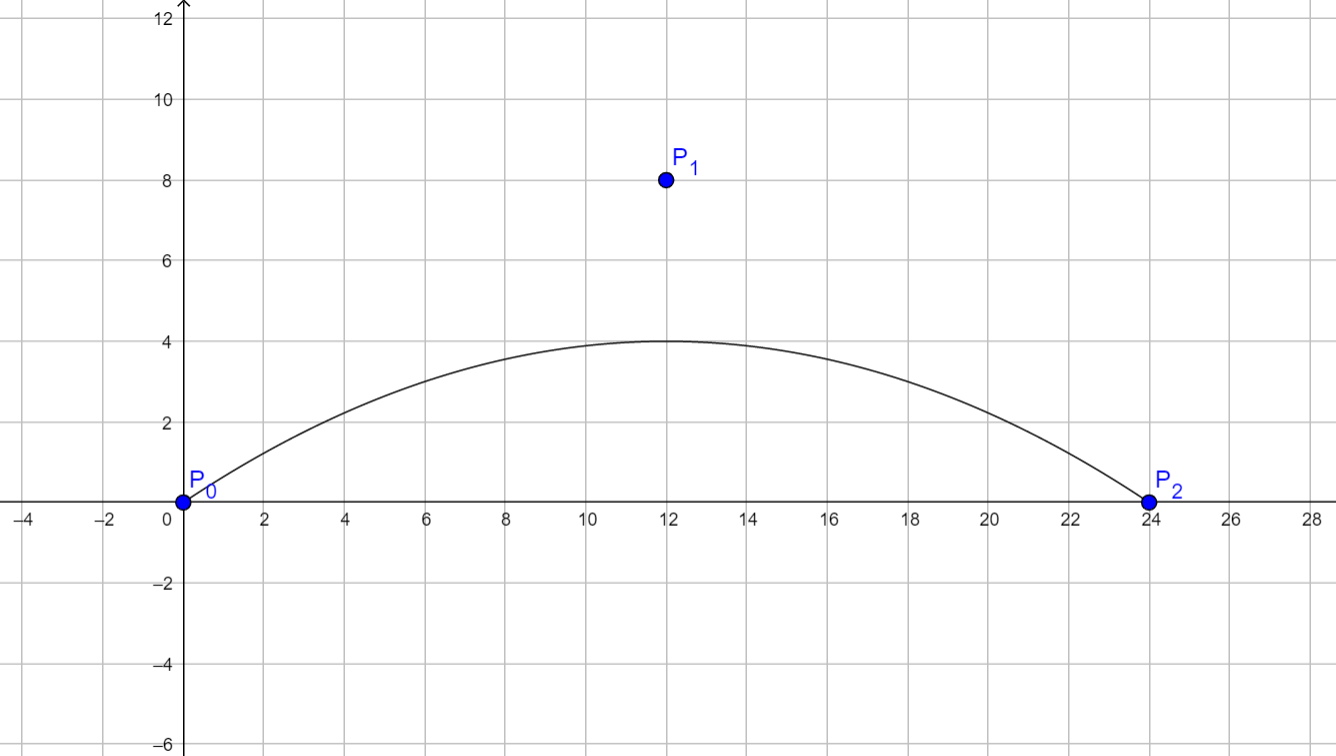
\includegraphics[width=0.5\linewidth]{figures/theory/bezier_curves/quadratic1.png} & 
            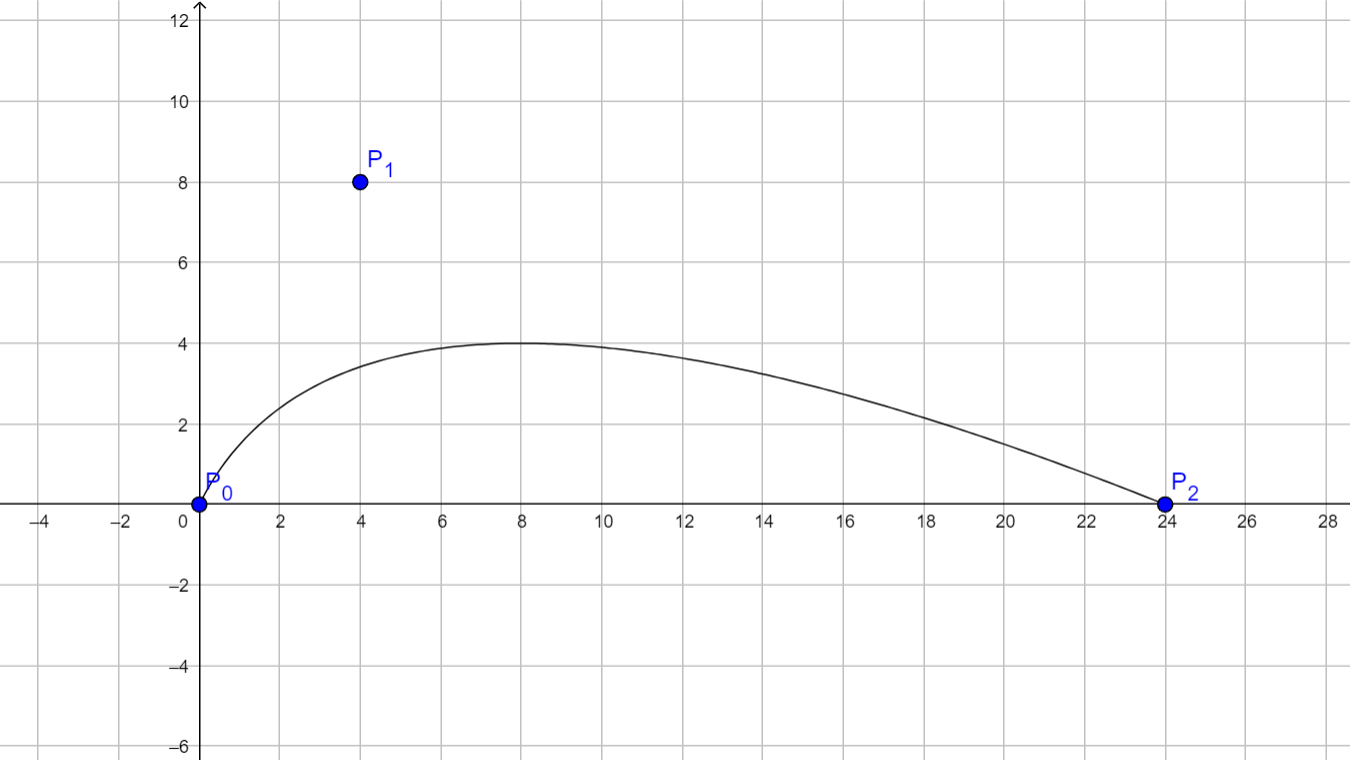
\includegraphics[width=0.5\linewidth]{figures/theory/bezier_curves/quadratic2.png} \\
            
            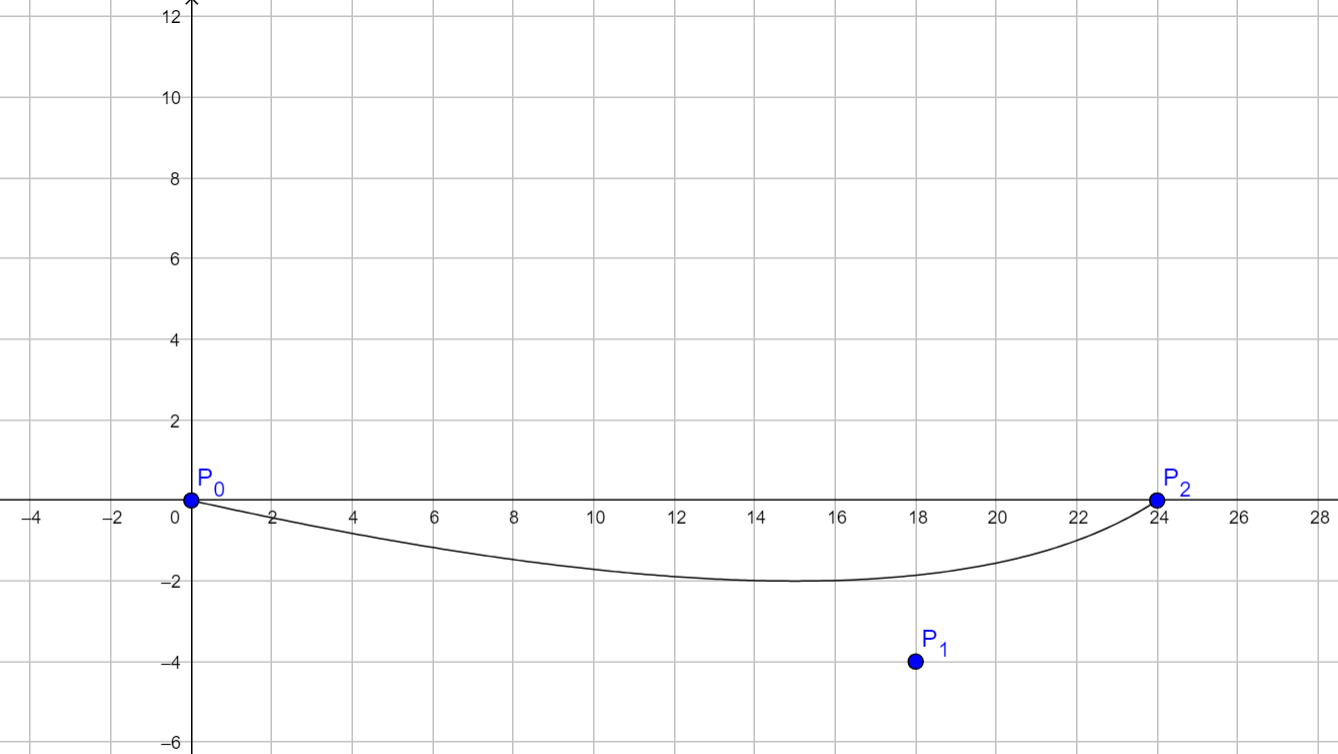
\includegraphics[width=0.5\linewidth]{figures/theory/bezier_curves/quadratic3.png} & 
            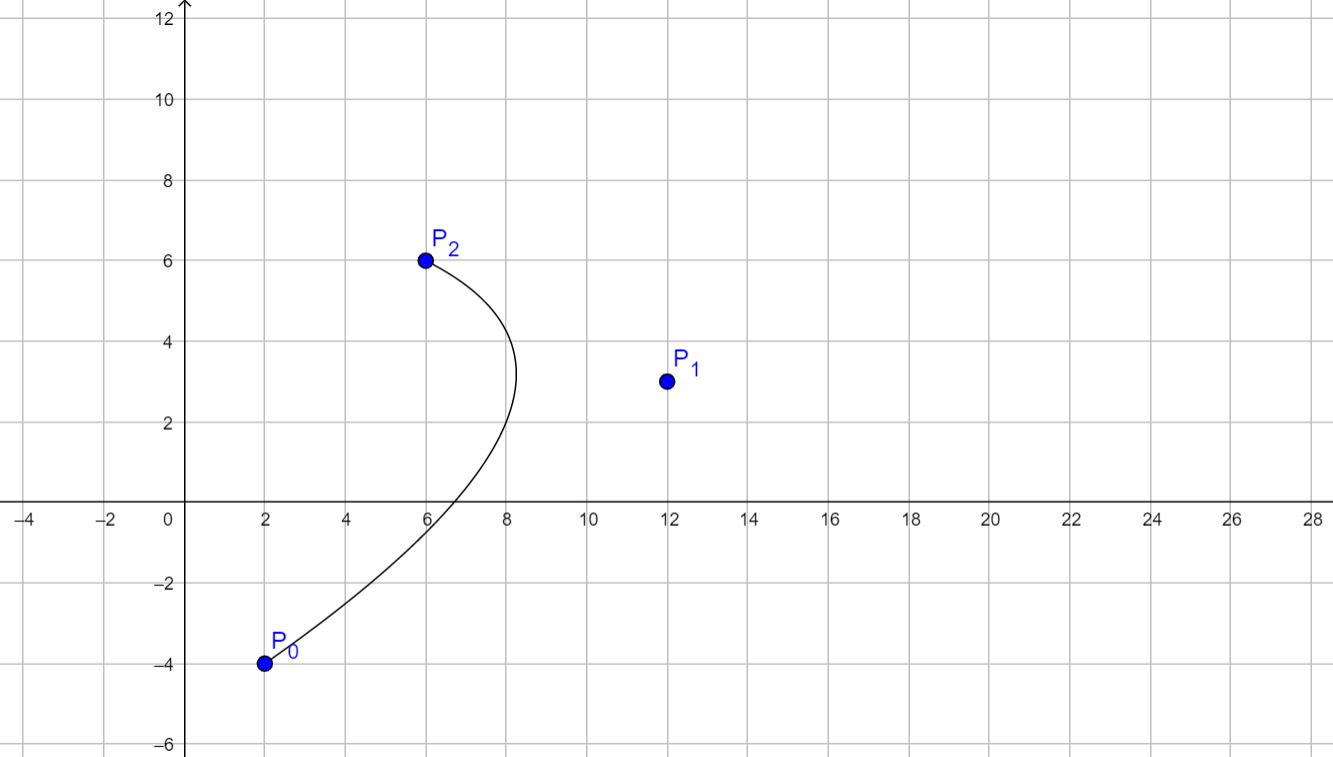
\includegraphics[width=0.5\linewidth]{figures/theory/bezier_curves/quadratic4.png}
        \end{tabular}
        \caption{Four examples of quadratic Bézier curves}
    \end{figure}

    
    
    % Hannes Kaulio and Marcus Schagerberg
    \subsection{Cubic Bézier Curve}
        A cubic Bézier curve expands on the quadratic curve in the same fashion as the quadratic expanded on the linear Bézier curve, adding another layer of linear interpolations. A cubic Bézier curve has four control points, two of which are endpoints.
        
        \inlineimage{figures/theory/bezier_curves/bezier_curve.png}{Cubic Bézier curve with control points \p{0}, \p{1}, \p{2} and \p{3}}{0.5}
    
        The cubic Bézier curve can be defined by the formula\cite{Cubic-Bézier-Curves}: 
        $$
            P(t) = (1-t)^3P_0 + 3t(1 - t)^2P_1 + 3t^2(1 - t)P_2 + t^3P_3 \timeconstraint
        $$
        Properties of the Cubic Bézier curve relevant to this paper are the following:
        \begin{enumerate}
            \item The endpoints \p{0} and \p{3} lay on the curve
            \item The curve is continuous, infinitely differentiable, and the second derivatives are continuous.
            \item The tangent line to the curve at the point \p{0} is the line \p{0}\p{1}. The tangent to the
        curve at the point \p{3} is the line \p{2}\p{3}.
            \item Both \p{1} and \p{2} lay on the curve only if the curve is linear.
            \item A Bézier curve is contained within the convex hull of the control points. For the application in Unity, this means that a Bézier curve is completely contained within the bounding box created by its control points.
        \end{enumerate}

    % Marcus Schagerberg
    \subsection{De Casteljau's algorithm}
        In 1959 the french mathematician Paul de Casteljau constructed an algorithm for dividing a Bézier curve into two. The union of these Bézier segments is equivalent to the original curve.
    
    % Marcus Schagerberg
    \subsection{Bézier Clipping}
        Finding the intersection points between two Bézier paths is not as straight forward as for something like two lines. To solve this, an algorithm called Bézier clipping explained in \cite{bezier-clipping} can be used. It utilises the convex hull property of Bézier curves - and therefore Bézier paths - as well as de Casteljau's algorithm for splitting curves. An implementation for finding all intersection points between two Bézier paths using Bézier clipping is outlined below.

        \vspace{1cm}
        \begin{algorithmic}
            \State $intersections \gets$ Empty list
            \State $epsilon \gets$ A value >0 small enough for the desired accuracy
            \Procedure{FindBezierPathIntersections}{$A, B$}
                \If{$A.BoundingBox$ does not intersect $B.BoundingBox$}
                    \State \Return
                \EndIf

                \If{$A.BoundingBox.Size$ + $B.BoundingBox.Size < epsilon$}
                    \State $intersections \gets$ Midpoint between A and B
                    \State \Return
                \EndIf

                \State $A_1, A_2 \gets SplitWithDeCasteljau(A, 0.5)$
                \State $B_1, B_2 \gets SplitWithDeCasteljau(B, 0.5)$

                \State $FindBezierPathIntersections(A_1, B_1)$
                \State $FindBezierPathIntersections(A_1, B_2)$
                \State $FindBezierPathIntersections(A_2, B_1)$
                \State $FindBezierPathIntersections(A_2, B_2)$
            \EndProcedure
        \end{algorithmic}
        \vspace{1cm}

        Worth noting is the $Midpoint$, which is one of many possible approximations of the intersection point. For a small enough $epsilon$, the approximation used is trivial as the segments approaches points as $epsilon$ approaches 0.

    % Hannes Kaulio and Marcus Schagerberg
    \subsection{Composite Bézier curve}
        A composite Bézier curve is a spline made out of Bézier curves. The series of Bézier curves are joined together end to end with the start point of one curve coinciding with the end point of the other curve. This is used in the projects as it allows for chaining of cubic Bézier path segments creating a spline. 

% Hannes Kaulio
\section{A* Algorithm}
    A* is an algorithm widely used for path finding and graph traversal \cite{A-Star-Algorithm}. It is classified as an informed search algorithm since it greedily explores the path finding environment by taking into account both the cost of the path from the starting node to the one that is currently being explored, as well as a heuristic function that estimates the distance between the currently explored node and the goal node. Given a start, and end node in a weighted graph, the algorithm will find the shortest path between the nodes. Together, these two forms an estimate function of the best path towards the goal. Given that A* is complete under the precondition that the search space is finite, and that the branching factor is finite as well, this guarantees that if a path exist, it will be found. Furthermore, if some additional conditions are fulfilled with regards to the heuristic function, A* can be guaranteed to return an optimal path. For this to be the case, the heuristic function needs to admissible or consistent, since a consistent function is also by definition, admissible. 

% Marcus Schagerberg
\section{Procedural mesh generation}
    All physical objects in Unity have an associated mesh, i.e. their surfaces. A cube for example can be thought of as having a mesh consisting of 6 different surfaces. In computer graphics, a triangle mesh is a type of mesh where the surfaces are created through a set of points, called vertices. These vertices are then joined together by a set of triangles. Going back to the cube example, a cube in its simplest form would have 12 triangles and 8 vertices. The eight vertices are at the corners of the cube. Each face of the cube has the shape of a square, which can be created with two triangles, hence double the amount of triangles as square faces.

\section{Scrum and Agile Software Development}
Agile Software Development is a software development framework which emphasizes vertical development cycles, where software should be delivered frequently in atomic slices to enable quick feedback and high flexibility with regards to how the product develops. When developing complex products, and especially when the development team has not worked on anything similar to the current developed product, implementing an Agile framework can be particularly important. Since features is delivered in small complete chunks, this minimizes the investment risk compared to a more horizontal feature development. 

\section{ABM}

